\section{Plan de gestión del proyecto}
\label{planes}
\subsection{Procesos}
\label{procesos}

El proyecto está dividido en dos iteraciones, cada una de ellas posee cinco fases: requisitos, análisis, diseño, implementacion y pruebas. En la primara iteración se va a desarrollar el funcionamiento de una partida tanto individual como por parejas y la página web con las pantallas de login y perfil de usuario. En la segunda iteración se va a desarrollar el resto de funcionalidades del sistema, que incluyen la inteligencia artificial, torneos, tienda, entre otros.  Cada fase de cada iteración tiene una duración máxima de una semana, excepto la fase de recogida de requisitos que tiene una duración inferior y que solo se lleva a acabo al inicio del proyecto.
A lo largo del proyecto el equipo se divide en los grupos de desarrollo: bases de datos y despliegue, backend, frontend y middelware e IA. En cada uno de ellos la participación es flexible pero se mantiene de forma fija a un responsable.

\subsubsection{Procesos de inicio del proyecto}
\label{inicio}

Al iniciar el proyecto, cada grupo de desarrollo adquiere las herramientas necesarias para el desarrollo del proyecto. Las principales herramientas son el entorno de desarrollo IntelliJ, creando una cuenta gratis de estudiante y una cuenta de GitHub para poder llevar a cabo el control de versiones del código y documentación del proyecto. Además, se adquiere un certificado TLS gratuito obtenido através del servicio "Let's Encrypt". \\

Además, el equipo  de bases de datos y despliegue debe registrarse en Amazon AWS con la cuenta de estudiante para la contratación de un servicio cloud en Amazon AWS y realizar un estudio para finalmente adquirir un dominio web.  Al finalizar el proyecto estos recursos son traspasados al cliente. \\

Si aparece algún otro recurso necesario cuya adquisición necesite una aportación económica debe ser notificado al director y aprobado por este antes de contratar dicho recurso.\\

Dado que el proyecto integra un gran número de tecnologías y capas que conforman la arquitectura web, es necesario realizar un estudio de viabilidad de las tecnologías escogidas antes de realizar la adquisición del software de desarrollo, este estudio requiere  5 horas de trabajo entre todos los grupos.  En un principio el desarrollo del proyecto se realiza sobre JavaEE, JSP, WebSockets, JavaScript, Bootstrap y MySQL. Como una parte del equipo de desarrollo posee cierta experiencia en el desarrollo web, no tanto en la utilización de estas herramientas, es necesario que se lleve a cabo un proceso de aprendizaje inicial. Este proceso requiere un número mínimo de horas para permitir al equipo comenzar con el desarrollo del proyecto. No obstante, a lo largo del proyecto la formación y la adquisición de experiencia son fundamentales.\\

En aquellas tecnologías donde el equipo de desarrollo no posee ninguna experiencia, como WebSockets, JavaScript , JSP,  entre otros, se requiere un esfuerzo extra por parte del equipo para auto-formarse mediante la lectura de libros, tutoriales y la documentación pertinente.\\

\begin{itemize}
	\item Tanto Carlos Marañés como Javier Corbalán se tienen que formar en Javascript, Websockets y Phaser.io a través del uso de ejemplos y documentación en línea.
	\item Julia Guerrero y Sergio Izquierdo deben formarse en HTML/CSS y JSP con documentación en línea y  con la ayuda de los miembros del equipo que tienen experiencia en esa tecnología.
    \item El equipo entero se va a formar en la dinámica de trabajo con AWS gracias a la experiencia de Sergio Izquierdo y tutoriales en línea.
\end{itemize}

\subsubsection{Procesos de ejecución y control del proyecto}

Una de las funciones más importantes del director del proyecto es gestionar la comunicación dentro del equipo. Para garantizar que esta máxima se cumple, el director tiene la capacidad de convocar reuniones que incluyan a todo el equipo o solo a los responsables de cada grupo de desarrollo. En cada reunión se realiza un acta que recoge todos los aspectos y decisiones importantes acaecidas en la reunión. Las decisiones tomadas en estas reuniones deben trasladarse a la documentación del proyecto y finalmente a la implementación.
\\\\
Los grupos de desarrollo se coordinan de forma autónoma para no sobrecargar la figura de director, para ello existe la figura de responsable, ya avanzada anteriormente. Si el equipo de trabajo sigue un correcto funcionamiento el director solo debe reunirse con los responsables de cada grupo, sin embargo en ocasiones extraordinarias puede reunirse con todo el grupo para tomar decisiones que engloben a todo el proyecto, o para corregir posibles funcionamientos incorrectos. Los objetivos globales de cada grupo son supervisados semana a semana por el director del proyecto. Mientras que dentro de cada grupo el responsable asigna día a día las tareas necesarias para cumplir con los objetivos. Los objetivos que semanalmente cada grupo de desarrollo se marca deben ser sencillos, concretos y trazables, de forma que permitan  medir semanalmente el progreso del proyecto.\\

En aquellas situaciones donde se requiera mediación, ya sean disputa o bajo rendimiento, el responsable del grupo de desarrollo debe intervenir realizando aquellas acciones que considere necesarias. En caso de disputa si su resolución no satisface a ambas partes, el director del proyecto junto con el responsable del grupo y las dos partes de la disputa se reunen para tomar las decisiones y resoluciones necesarias para finalizar la disputa.\\

El proyecto se almacena en un repositorio central donde se lleva el control de versiones. Al finalizar el proyecto se otorga al cliente el repositorio, el codigo fuente y el control de la aplicación ya desplegada. Al final de cada semana se debe estudiar el progreso del proyecto según las pautas marcadas en el diagrama de Gantt, pudiendo revisar y actualizar dicho diagrama.

\subsubsection{Procesos técnicos}

La generación de documentación del sistema se llevará a cabo por el propio equipo de desarrollo durante la implementación de la aplicación. Esta documentación será almacenada y actualizada dentro del repositorio central. Para generar la documentación general se seguirá el estandar UML utilizando la herramienta StarUML en su versión de prueba. En el caso de las diferentes clases y paquetes que componen el sistema se utilizarán las herrramientas disponibles para generar la documentación automáticamente como Javadoc y JSdoc.

Para el desarrollo de los diferentes paquetes y componentes que componen el sistema se sigue la metodología de programación en parejas. Donde dos personas construyen una misma clase, uno escribe el código fuente mientras que el otro supervisa la corrección del código. A lo largo del proyecto cada equipo de desarrollo utiliza diferentes herramientas de desarrollo para falicitar la implementación del proyecto, la gestión de versiones y la compilación o interpretación de cada lenguaje utilizado. En general se utlizan los IDEs de JetBrains. IntelliJ IDEA para Java, WebStorm para JS, DataGrip para SQL y modelado de la base de datos.

El despliegue de la aplicación se lleva a cabo utilizando los servicios de Amazon AWS que facilitan un despliegue rápido y sencillo.

\subsection{Planes}
\label{pl}
\subsubsection{Plan de gestión de configuraciones}
\begin{itemize}
		% \item \textbf{Convenciones de nombres (documentos) y estándares de código.}
    \item La documentación está centralizada en un repositorio online. Se divide en varios archivos fuente de \LaTeX~ en función de las secciones del documento. De este modo existen los siguientes archivos:
		\begin{itemize}
			\item \textit{main.tex:} Contiene las macros de la documentación, la introducción y la estructura del resto del documento.
			\item \textit{2-organización.tex:} Contenido de la Sección \textit{Organización del Proyecto}.
			\item \textit{3-gestion.tex:} Contenido de la Sección \textit{Plan de Gestión del Proyecto}.
			\item \textit{4-analisis-diseno.tex:} Contenido de la Sección \textit{Análisis y Diseño del Sistema}.
			\item \textit{5-memoria.tex:} Contenido de la Sección \textit{Memoria del Proyecto}.
			\item \textit{data.bib:} Base de Datos con la bibliografía usada.
		\end{itemize}
		Las imágenes, figuras y diagramas que se utilizan desde esos archivos están guardadas en la carpeta \textit{figuras} con un nombre descriptivo. Además existe una versión compilada (PDF) de la última versión de los documentos así como los documentos anteriormente entregados con el nombre \textit{main-aaaa-mm-dd.pdf}.

		La \textit{Propuesta Técnica y Económica} está disponible en formato Word en el fichero \textit{propuesta.docx} al igual que su documento compilado (PDF) y los documentos anteriormente entregados con el nombre \textit{propuesta-aaaa-mm-dd.pdf}

		Las actas de reuniones están en la carpeta \textit{actas} y sus nombres siguen el patrón \textit{acta-aaaa-mm-dd}.

		La contabilidad de las horas de trabajo empleadas por cada miembro del equipos se encuentran en un fichero de cálculo llamado \textit{contabilidad-horas}.
 \item{ Para llevar un control de las versiones del código se crea un repositorio central en la misma organización de GitHub que la documentación y se utiliza el gestor de incidencias integrado en GitHub para resolver errores.}
\item{Cada responsable de equipo designa las tareas de los miembros de su equipo utilizando el gestor de tareas propio de GitHub. }

    % \item\textbf{ Responsable o responsables de las distintas actividades (puesta en marcha, apoyo al equipo, revisión de commits, copias de seguridad, control de las versiones entregadas a cliente...).}
\item{Se deben realizar commits frecuentes siempre que el código compile. Los commits deben representar avances lógicos y atómicos de trabajo.  Si el código subido afecta al de los compañeros se debe crear una incidencia para notificarles  y recibir aprobación del resto del equipo para realizar el commit. Al programar en parejas, la revisión de los commits por parte de los compañeros de equipo (en parejas o tríos) se produce de forma natural. Los responsables de equipo son los encargados de realizar una copia de seguridad semanal off-site de su parte del repositorio mientras que el director del proyecto la debe realizar del repositorio completo. El director también es el responsable directo del control de las versiones entregadas al cliente. }
    % \item \textbf{Recursos: repositorios de control de versiones (cuáles, cuántos, permisos de acceso a los mismos) y sistema de gestión de incidencias.}
    % \item \textbf{Procedimiento para realizar cambios al código fuente y los documentos técnicos: workflow de control de versiones utilizado, cuándo/cómo se permiten realizar commits al repositorio compartido, si tienen que ser aceptados por alguien previamente o no, qué hay que anotar en el sistema de gestión de incidencias, quién decide el estado de las incidencias, en qué estados puede estar una incidencia etc.}
		\item Los equipos realizan su trabajo sobre una rama basada en la rama central del repositorio (rama del equipo). Los miembros de los equipos realizan los commits sobre la rama del equipo (aunque pueden tener ramas auxiliares basadas en la rama del equipo). El responsable de cada equipo es quien puede incluir los avances hechos sobre una rama de equipo en la rama central del repositorio.
\end{itemize}

\subsubsection{Plan de construcción y despliegue del software}

La construcción del software se desarrolla con la utilización del framework Intellij IDEA.\\

El software se despliega en tres niveles. El cliente, utilizando un navegador Chrome, interactua con el software desplegado en el servidor web, a través de una conexión https. El servidor web mantiene  el puerto 443 abierto para permitir las conexiones https efectuadas por los clientes. El software del servidor web se despliega en Amazon AWS, en una instancia de EC2, y este interactúa con la base de datos desplegada en Amazon Aurora para la creación de partidas o la modificación de los datos de un jugador. La comunicación entre el servidor web y la base de datos se desarrollara en una intranet utilizando la API JDBC que permite la ejecución de operaciones sobre bases de datos.

\begin{figure}[H]
\centering
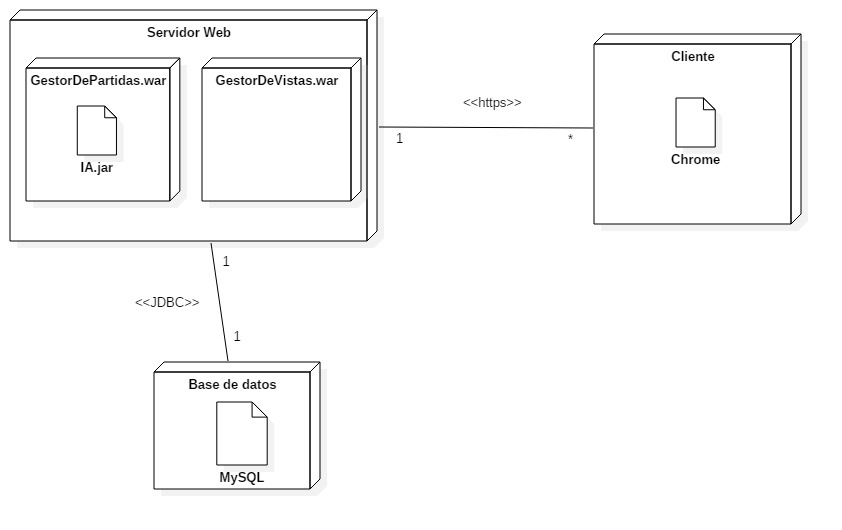
\includegraphics[scale = 0.4]{figuras/despliegue.jpg}
\caption{Diagrama de despliegue}
\label{fig:diagramaDespliegue}
\end{figure}

\subsubsection{Plan de aseguramiento de la calidad}

Uno de los pilares del proyecto es el control de la calidad del software. Para ello el equipo intenta automatizar las tareas a este respecto todo lo posible y apoyarse en los siguientes pilares:
\begin{itemize}
\item{Para garantizar el correcto funcionamiento de los paquetes, clases y funciones generados se realizan diferentes test unitarios. Para las clases cuyos métodos están formados por bucles complejos o varios condicionales se realizan pruebas de caja blanca utilizando la técnica de análisis de caminos. Para el resto de métodos no triviales se realizan pruebas de caja negra con clases de equivalencias y análisis de valores del límite para aquellos métodos que resuelven problemas con valores pertenecientes a unos rangos concretos. Para las pruebas unitarias en Java y Javascript, se utilizan JUnit y unit.js respectivamente. Estas pruebas deben ser satisfactorias antes de cada commit para, adicionalmente, dar un mínimo de garantías de funcionamiento correcto del código que se almacena en el repositorio.\\ Además, uno de los integrantes del equipo se va a dedicar a realizar pruebas manuales jugando varias partidas en un simulador en las fases iniciales del proyecto y en el sistema real una vez implementado.}
\item{Para la integración de los diferentes módulos entre sí, se realizan test de integración.}
\item{Como guías de estilo, se utilizan las de Google para Java, Javascript, HTML y CSS. En el caso de que a lo largo del desarrollo se introduzca algún lenguaje nuevo, los responsables de equipo y el director consensúan el uso de una guía de uso concreta. En caso de no existir una, se crea un documento con directivas importantes a seguir al utilizar ese lenguaje.}
\item{Para representar y especificar el sistema tanto dentro como fuera de la organización, se utiliza el estándar UML, agilizando y concretando la comunicación entre equipos, evitando errores causados por una mala comprensión de la arquitectura del sistema.}
\item{Se programa por parejas las partes críticas de la lógica del juego y de la aplicación para reducir el número de errores y mejorar la calidad del código en general.}
\item{Cada 30 días se realiza una revisión de requisitos de la aplicación en la que se especifican los requisitos cumplidos y los pendientes.}
% \item  \textbf{Estándares de código y otros (se pueden definir guías para la documentación de diseño y otros documentos del proyecto).}
%     \item \textbf{ Actividades de control de calidad del código que se realizarán: revisiones de código por pares, revisiones de requisitos o diagramas UML por pares, tipos de tests automáticos o manuales que se llevarán a cabo.}
\end{itemize}
\subsubsection{Calendario del proyecto y división del trabajo}
	\begin{figure}[H]
		\hspace{-3cm}
		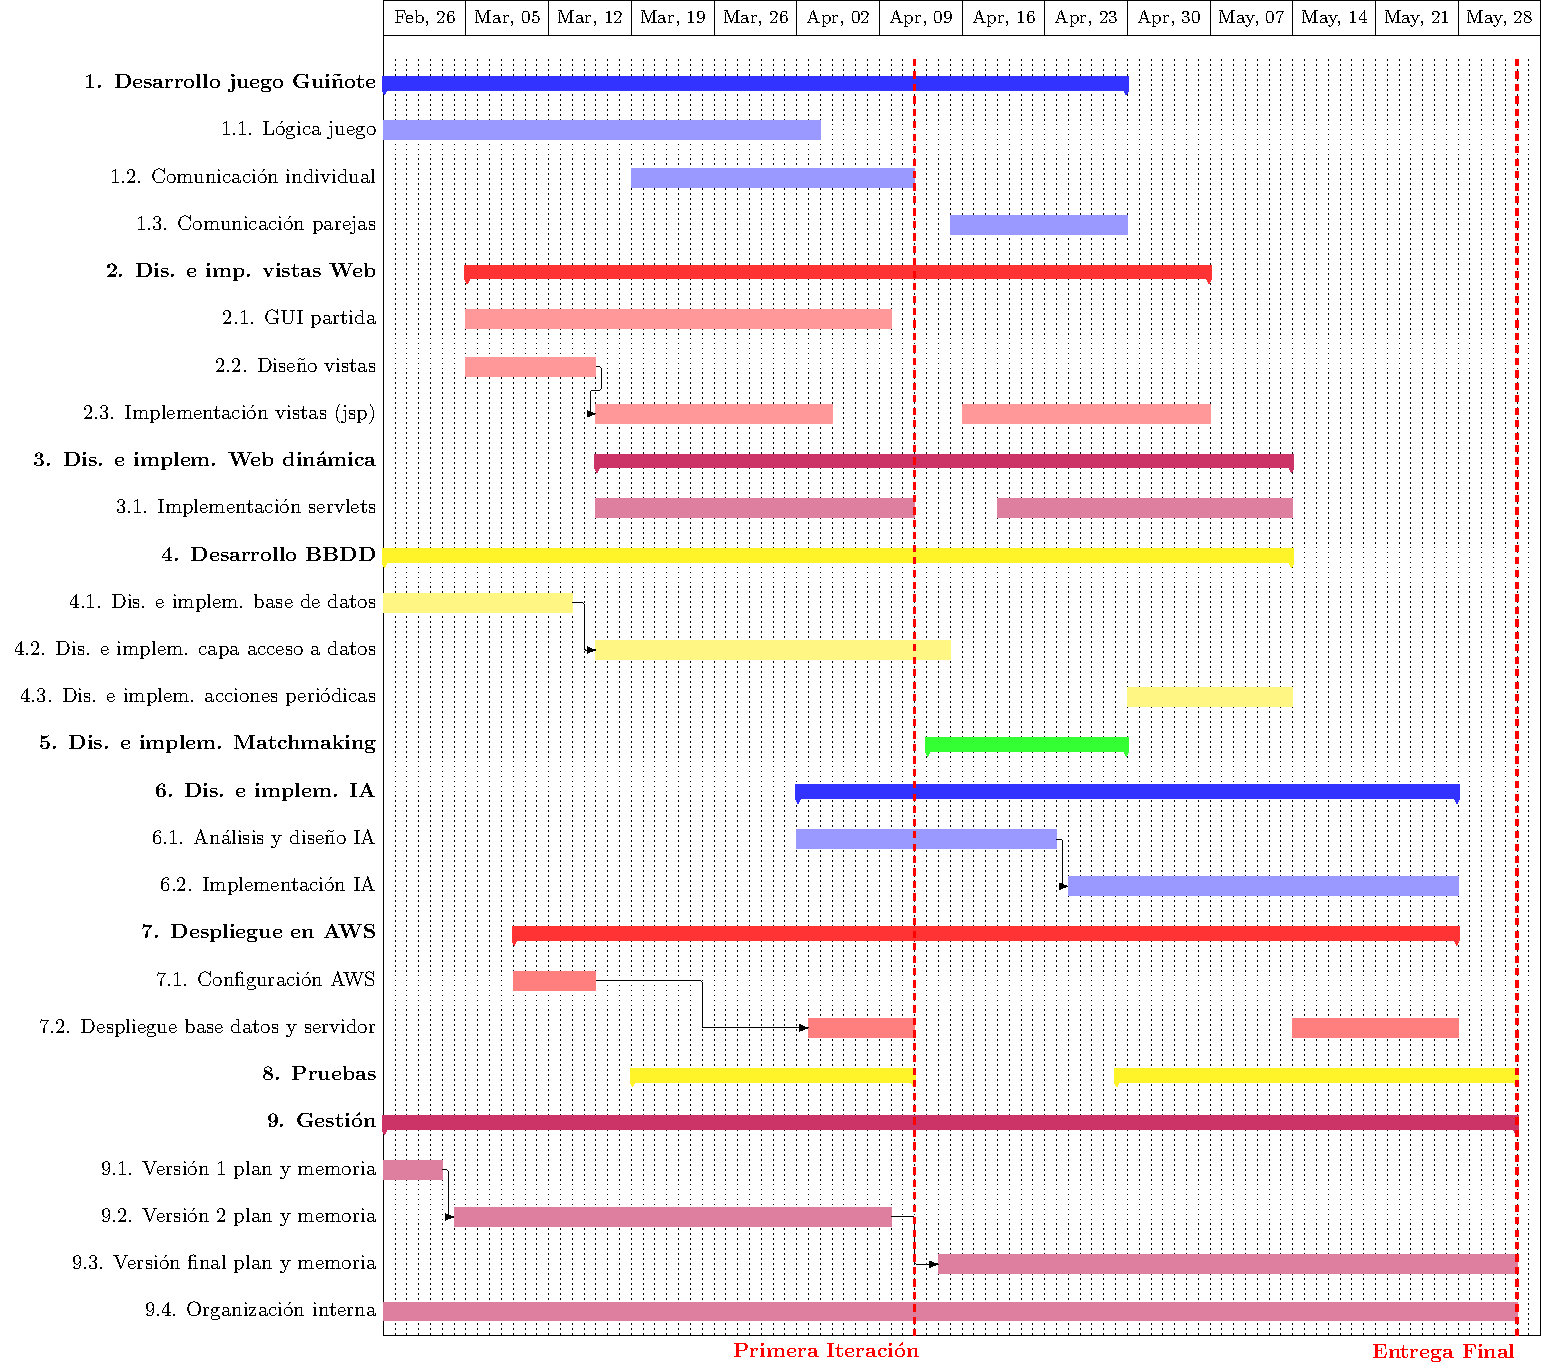
\includegraphics[scale=0.8]{figuras/gantt.pdf}
		\caption{Diagrama de Gantt}
	\end{figure}
% \begin{itemize}
%     \item\textbf{ Diagrama de Gantt que recoja las tareas a realizar. Tened en cuenta que trabajáis con dos iteraciones y por tanto que hay una entrega intermedia y una final, y reflejarlo en este diagrama. Tened en cuenta que es normal que lo tengáis que actualizar conforme avance el proyecto (cuándo y cómo establezcáis en la sección 3.1.2).}
%      \item \textbf{Debe quedar claro qué requisitos van a estar completados en la primera iteración y cuáles en la segunda. Es posible que para la primera iteración no se planifique completar ningún requisito, pero en ese caso tiene que planificarse qué se hará y que faltará por hacer para cada requisito.}
%     \item \textbf{División del trabajo en partes (los módulos del software a desarrollar, pero también  la documentación, el diseño gráfico, instalaciones o despliegues, pruebas manuales etc.) y reparto de los mismos entre el equipo de desarrollo, al menos a alto nivel (el reparto de labores concretas en el día a día no se detalla aquí, pero hay que explicar bajo qué criterios y quién/cómo se hace en la sección 3.1.2). Debe haber una correspondencia con las tareas que aparecen en el diagrama de Gantt (que no necesariamente tiene que ser una relación 1 a 1).}
%      \item \textbf{Verificar que esta división del trabajo cubre todos los requisitos}
% \end{itemize}

Como se observa en el diagrama, el proyecto está dividido en dos iteraciones, con sus correspondientes demostraciones al cliente del avance del proyecto. La primera iteración finaliza la semana del 9 de abril y la segunda, que se corresponde con la entrega final, el 1 de junio.\\

%TODO: terminar esta sección cuando marius acabe los requisitos (cambiando los numeros o quizas hablando de bloques de requisitos)
\textbf{Primera iteración}

En la primera iteración se presenta una partida funcional individual, así como la página web con las vistas de las pantallas de login y perfil de usuario. También esta disponible el modo espectador. La inteligencia artificial está analizada pero no implementada todavía.

En concreto, los requisitos funcionales 2-6, 9-10 y los requisitos no funcionales 1-2 está cubiertos completamente. Además, el requisito funcional 1 está cubierto en cuanto a las partidas individuales, pero queda la implementación de las partidas por parejas. El requisito funcional 13 está cubierto parcialmente, ya que los turnos tienen un periodo de tiempo establecido, acabando la partida si el jugador no realiza movimiento, pero el sistema de puntuaciones no esta implementado.
De la misma forma, relativo a los requisitos funcionales 14 y 17, se puede abandonar la partida manualmente pero todavía no hay penalización de puntuaciones. Finalmente, el requisito funcional 24 correspondiente al desarrollo de la inteligencia artificial, queda cubierto solo parcialmente, en lo que respecta a análisis y representación del problema pero no la implementación e integración con el resto del sistema.\\

\textbf{Segunda iteración}

En la segunda iteración o entrega final, se presenta al cliente el sistema con todas las características especificadas totalmente funcionales. Se añaden a las funcionalidades de la primera iteración todas las correspondientes a las puntuaciones, las ligas y los torneos (así como su programación automática), el sistema de matchmaking, la tienda, el panel de administración y la inteligencia artificial.

En concreto, se cubren por completo los requisitos funcionales 1, 7-8, 11-24 y los no funcionales 3-7.


\subsubsection*{División del trabajo}
\label{repartotrabajo}
A continuación, se detalla una división del proyecto en bloques, con el correspondiente equipo o equipos de los descritos en la sección \ref{organiz} que los lleva a cabo. Además, se incluye la lista de requisitos (especificados en el apartado \ref{requisitos}) que quedan cubiertos en cada uno de estos bloques para garantizar que se satisfacen todos ellos.
%TODO: terminar con los requisitos

\begin{table}[H]
\label{divisionTrabajo}
\hspace{-0.8cm}
\begin{tabular}{|l|c|l|}
\hline
\multicolumn{1}{|c|}{\textbf{Bloque}}                          & \textbf{Equipo} & \multicolumn{1}{c|}{\textbf{Requisitos}}                                                                       \\ \hline
Desarrollo de la interfaz del guiñote                 & 1      & \begin{tabular}[c]{@{}l@{}}\small{RF: 1,6}\\ \small{RNF: 2}\end{tabular}                                              \\ \hline
Desarrollo de la lógica de juego del guiñote          & 4      & \begin{tabular}[c]{@{}l@{}}\small{RF: 1}\\ \small{RNF: -}\end{tabular}                                                \\ \hline
Diseño e implementación de vistas web                 & 1      & \begin{tabular}[c]{@{}l@{}}\small{RF: 2,4,6,7,8,9,11,15,18,19,20,21}\\ \small{RNF: 2}\end{tabular}                    \\ \hline
Implementación de la web dinámica                     & 4      & \begin{tabular}[c]{@{}l@{}}\small{RF: 1,6,12,13,14,16,17}\\ \small{RNF: 3,5}\end{tabular}                             \\ \hline
Diseño e implementación de las comunicaciones         & 1      & \begin{tabular}[c]{@{}l@{}}\small{RF: 1,3,4,12}\\ \small{RNF: 1,2}\end{tabular}                                       \\ \hline
Desarrollo de la base de datos                        & 2      & \begin{tabular}[c]{@{}l@{}} \small{RF: 2,4,7,9,11,13,14,15,16,17,18,19,20,22,23}\\ \small{RNF: 1,3,4,5,6}\end{tabular} \\ \hline
Diseño e implementación de la Inteligencia Artificial & 3      & \begin{tabular}[c]{@{}l@{}}\small{RF: 24}\\ \small{RNF: -}\end{tabular}                                               \\ \hline
Despliegue                                            & 2      & \begin{tabular}[c]{@{}l@{}}\small{RF: 10}\\ \small{RNF: 1}\end{tabular}                                               \\ \hline
\end{tabular}
\caption{Tabla de división del trabajo}
\end{table}
